\documentclass[../main/main.tex]{subfiles}

\begin{document}

\setcounter{chapter}{1}
\chapter{Miroirs et dioptres plans}
\vspace*{-47pt}
\begin{center}
    \Huge Exercices d'application
\end{center}

\section{Miroir plan et tracé des rayons}
\subsection{}
\begin{minipage}{0.75\linewidth}
    On a intersection des rayons incidents avant le miroir, c'est un objet réel.
    L'image de cet objet par le miroir est son symétrique par rapport au plan du
    miroir : elle est virtuelle. Les rayons émergents passent par cette image
    (mais sont en pointillés derrière le miroir).
\end{minipage}
\begin{minipage}[c]{0.25\linewidth}
    \begin{flushright}
        \includegraphics{../figures/ch2-1-1}
    \end{flushright}
\end{minipage}

\subsection{}
\begin{minipage}{0.75\linewidth}
    Les rayons incidents se croisent après le miroir. On a un objet virtuel. Son
    image par le miroir plan est son symétrique par rapport au plan du miroir.
    C'est donc une image réelle (au-dessus du miroir). Les rayons émergents
    passent par cette image.
\end{minipage}
\begin{minipage}{0.25\linewidth}
    \begin{flushright}
        \includegraphics{../figures/ch2-1-1}
    \end{flushright}
\end{minipage}

\subsection{}
\begin{minipage}{0.75\linewidth}
    Ici on a des rayons émergents. Leur intersection est, par définition, le
    point image. Elle se fait derrière le miroir : c'est un image virtuelle. On
    obtient l'objet associé en en faisant le symétrique par rapport au plan du
    miroir : il est donc au-dessus, et c'est un objet réel.
\end{minipage}
\begin{minipage}{0.25\linewidth}
    \begin{flushright}
        \includegraphics{../figures/ch2-1-3}
    \end{flushright}
\end{minipage}

\section{Une grenouille intelligente}
\begin{tcbraster}[raster columns=7, raster equal height=rows]
    \begin{NCdefi}[raster multicolumn=4]{Données}
        Pour une hauteur de grenouille fixée, il y a une taille de
        nénuphar permettant à tous les rayons partant de la grenouille de ne
        pas traverser le dioptre.\smallbreak
        \begin{center}
            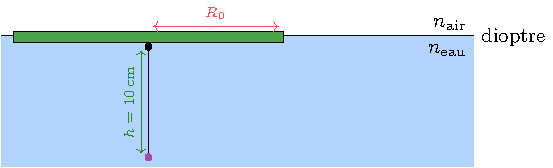
\includegraphics{../figures/ch2-2-1}   
        \end{center}
    \end{NCdefi}
    \begin{tcolorbox}[blankest, raster multicolumn=3, space to=\myspace]
        \begin{tcbraster}[raster columns=1]
            \begin{NCprop}{But à atteindre}
                Origine physique de ce phénomène et traduction mathématique.
            \end{NCprop}    
            \begin{NCdemo}{Outils du cours}
                Loi de Snell-Descartes :
                \[ n_1\sin i_1 = n_2\sin i_2\]
                et \underline{angle limite} de réfraction, tel que :
                \[ n_1\sin i_\ell = n_2\sin 90\degres = n_2\]
                qui indique que pour $n_1 > n_2$, il y a un angle d'incidence à
                partir duquel il n'y a pas de rayon réfracté (les rayons
                réfractés font un angle de 90° avec la normale et sont donc
                parallèles au dioptre).
            \end{NCdemo}
        \end{tcbraster}
    \end{tcolorbox}
\end{tcbraster}

\begin{NCexem}[breakable]{Application}
    Pour que les pieds de la grenouille ne soient pas visibles par un prédateur
    situé en-dehors de l'eau, c'est-à-dire au-dessus du dioptre, il faut
    simplement qu'il n'y ait pas de rayon partant de ses pieds et qui puissent
    sortir de l'eau : il faut que tous les rayons avec un angle d'incidence plus
    faible que cet angle limite soient bloqués par le nénuphar. C'est possible
    puisqu'on est dans une situation où le rayon passe dans un milieu
    \textbf{moins réfringent}, i.e. $n_2 < n_1$. En effet, dans cette situation
    il y a une inclinaison du rayon incident qui implique que le rayon émergent
    est parallèle à la surface, et tous les rayons au-delà de cet angle limite
    sont tous réfléchis. Un beau, grand schéma avec toutes les données reportées
    dessus mène naturellement à l'utilisation de formules trigonométriques de
    4$^\text{ème}$.
    \begin{center}
        \vspace*{-2.5cm}
        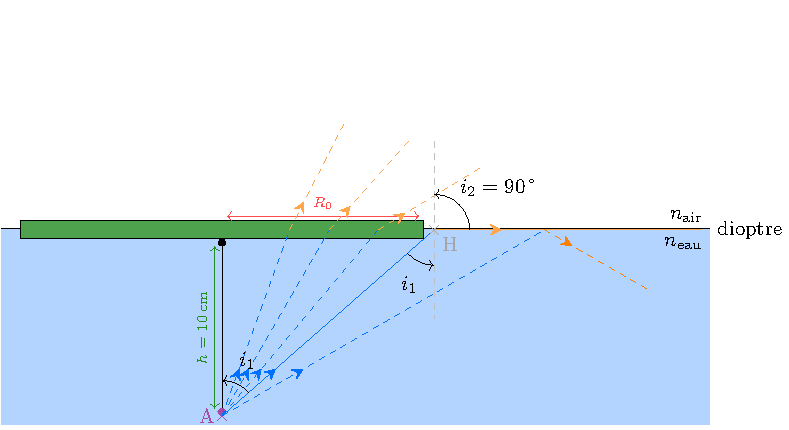
\includegraphics{../figures/ch2-2-2}
    \end{center}
    On voit ici qu'une simple fonction $\tan$ permet d'exprimer $R_0$ :
    \begin{empheq}[box=\fbox]{align}\label{eq:tan}
        \tan i_1 = \frac{R_0}{h}
    \end{empheq}
    Seulement on n'a pas encore la valeur de $i_1$. Or, on a déterminé que pour
    fonctionner l'astuce de la grenouille est d'avoir $i_1 = i_\ell$, et d'après
    le cours :
    \begin{empheq}{align}
        n\eau\sin i_\ell       & = n\air\\
        \Leftrightarrow i_\ell & = \asin \frac{n\air}{n\eau}\label{eq:ilim}
    \end{empheq}
    On peut donc écrire, avec \ref{eq:tan} et \ref{eq:ilim} :
    \begin{empheq}[box=\fbox]{equation}
        R_0 = h\times\tan\left(\asin \frac{n\air}{n\eau}\right)
        \quad \text{avec}
        \left\{
            \begin{array}{rcl}
                h & = & \SI{10.0}{cm}\\
                n_\mathrm{air} & = & 1\\
                n_\mathrm{eau} & = & 1.33
            \end{array}
        \right.
    \end{empheq}
    et finalement,
    \begin{empheq}[box=\fbox]{equation}
        R_0 = \SI{11.4}{cm}
    \end{empheq}
\end{NCexem}

\begin{tcbraster}[raster columns=3, raster equal height=rows]
    \begin{NCcoro}[raster multicolumn=2]{Conseil}
        Pour retenir vos formules trigonométriques, un moyen mnémotechnique :
        \begin{center}
            CAH\quad SOH \quad TOA
        \end{center}
        pour \[
            \cos\a = \frac{ \text{adjacent}}{ \mathrm{hypothénuse}} \quad
            \sin\a = \frac{ \text{opposé}}{ \mathrm{hypothénuse}} \quad
            \tan\a = \frac{ \text{opposé}}{ \mathrm{adjacent}} \]
    \end{NCcoro}
    \begin{NCimpo}{Important !}
        La deuxième plus \underline{grosse} erreur facile à faire mais cette
        fois pire que \textbf{tout}, c'est d'oublier que :
        \begin{center}
            \large \bfseries
            Les angles de la relation de Descartes sont définis entre les
            rayons et la \underline{normale} au dioptre !
        \end{center}
        Il ne faut pas prendre la surface du dioptre comme référence pour
        définir des angles.
    \end{NCimpo}
\end{tcbraster}

\newpage
\section{Le chat et le poisson}
\begin{tcbraster}[raster columns=3, raster equal height=rows]
    \begin{NCdefi}[raster multicolumn=2, sidebyside]{Données}
        \begin{enumerate}
            \item Aquarium $\equiv$ dioptre plan ;
            \item $n _\mathrm{eau} = 1.33$, $n _\mathrm{air} = 1$ ;
            \item $\obar{HA} = \SI{-15}{cm}$.
        \end{enumerate}
        \tcblower
        \begin{center}
            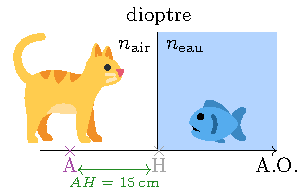
\includegraphics{ch2-3-1}
        \end{center}            
    \end{NCdefi}    
    \begin{NCprop}{Résultats attendus}
        \begin{enumerate}
            \item Sachant que le poisson observe la lumière partant du chat (point
                A), que vaut $\obar{HA'}$ ?
            \item Sachant que le \underline{chat} observe la lumière partant du poisson
                (point A), que vaut $\obar{HA'}$ ?
        \end{enumerate}
    \end{NCprop}
\end{tcbraster}

\begin{tcbraster}[raster columns=4, raster equal height=rows]
    \begin{NCdemo}{Outils du cours}
        Relation de conjugaison pour un objet $A$ dans un milieu d'indice $n_1$,
        dont l'image $A'$ est dans un milieu d'indice $n_2$ :
        \[ \frac{\obar{HA'}}{\obar{HA}} = \frac{n_2}{n_1}\]
        \begin{center}
            ou
        \end{center}
        \[\frac{\obar{HA'}}{n_2} - \frac{\obar{HA}}{n_1} = 0 \]
        \begin{center}
            ou
        \end{center}
        \[ 0 = \frac{n_2}{\obar{HA'}} - \frac{n_1}{\obar{HA}} \]
        qui ressemble « bizarrement » à la relation de conjugaison pour une
        lentille mince...
    \end{NCdemo}    
    \begin{NCexem}[raster multicolumn=3]{Application}
        \begin{enumerate}
            \item Dans ce cas, $A$, le chat, est dans un milieu d'indice $n_1 =
                1$ ; son image par le dioptre plan donne $A'$ dans le milieu
                d'indice $n_2 = n _\mathrm{eau} = 1.33$. On prend le sens de la
                lumière de l'objet à l'observataire, donc ici de gauche à
                droite. On adapte la relation de conjugaison :
                \[ \obar{HA'} = n _\mathrm{eau}\obar{HA} = \SI{-22.5}{cm}\]
                Ainsi, du point de vue du poisson, le chat est plus loin qu'il
                ne l'est vraiment.
            \item Dans ce cas, $A$, le poisson, est dans un milieu d'indice $n_1
                = n _\mathrm{eau} = 1.33$, et son image par le dioptre donne
                $A'$ dans l'air d'indice $n_2 = n _\mathrm{air} = 1$. Ici le
                sens de progagation est de droite à gauche. On réutilise la
                relation de conjugaison :
                \[ \obar{HA'} = \frac{\obar{HA}}{n _\mathrm{eau}} > \obar{HA} \]
                En effet, puisqu'on a posé le sens de propagation de droite à
                gauche, $\obar{HA} < 0$, et donc $\obar{HA'} > \obar{HA}$ comme
                $n\eau > 1$. Cela signifie que du point de vue du chat, le
                poisson est plus près du dioptre qu'il ne l'est vraiment.
        \end{enumerate}
    \end{NCexem}
\end{tcbraster}

\begin{NCexem}[sidebyside]{Schémas}
    \begin{center}
        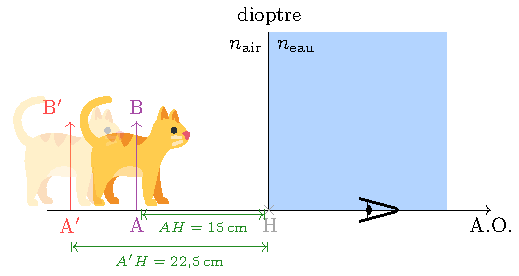
\includegraphics{ch2-3-2}
    \end{center} 
    \tcblower
    \begin{center}
        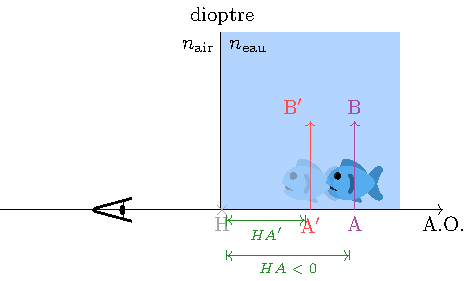
\includegraphics{ch2-3-3}
    \end{center} 
\end{NCexem}

\begin{tcbraster}[raster columns=5, raster equal height=rows]
    \begin{NCcoro}[raster multicolumn=2]{Conseils}
        Réécrire les formules telles que vous les avez apprises en cours,
        \textbf{puis} inclure les données de l'énoncé une par une pour éviter les
        erreurs...
    \end{NCcoro}    
    \begin{NCimpo}[raster multicolumn=3]{Important}
        \begin{enumerate}
            \item Ne pas se tromper sur le caractère {\huge algébrique} des
                grandeurs ;
            \item Bien identifier quelle est la source, quæl est l'observataire.
        \end{enumerate}
    \end{NCimpo}
\end{tcbraster}

\section{Champ de vision à travers un miroir plan}
\subsection{Propre image}
\begin{tcbraster}[raster columns=2, raster equal height=rows]
    \begin{NCdefi}{Schéma}
        \begin{center}
            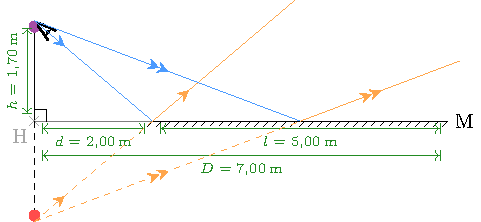
\includegraphics{ch2-4-1}
        \end{center}
    \end{NCdefi}
    \begin{tcolorbox}[blankest, raster multicolumn=1, space to=\myspace]
        \begin{tcbraster}[raster columns=1]
            \begin{NCdemo}{Outil}
                Pour voir une image, il faut qu'un rayon partant de l'image
                puisse arriver jusqu'à l'œil de l'observataire. Étant donné
                qu'on travaille avec un miroir, l'image de l'observataire est
                son symétrique par le plan du miroir (même si le miroir ne
                s'étend pas jusque-là !).
            \end{NCdemo}
            \begin{NCexem}{Application}
                On voit vite qu'il n'est pas possible qu'un rayon issu de
                l'image (en rouge) atteigne l'œil (en violet). On comprend par
                le tracé des rayons réfléchis que seul l'autre côté du lac sera
                visible.
            \end{NCexem}
        \end{tcbraster}
    \end{tcolorbox}
\end{tcbraster}

\subsection{Image arbre}
\begin{tcbraster}[raster columns=2, raster equal height=rows]
    \begin{NCdefi}{Schéma}
        \begin{center}
            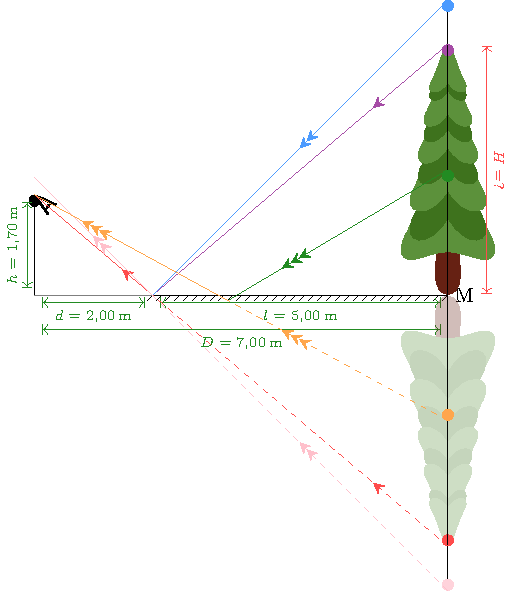
\includegraphics{ch2-4-2}
        \end{center}
    \end{NCdefi}
    \begin{tcolorbox}[blankest, raster multicolumn=1, space to=\myspace]
        \begin{tcbraster}[raster columns=1]
            \begin{NCdemo}[add to natural height=\myspace]{Outil}
                Ici aussi, l'idée est de trouver l'image de l'arbre, et de voir
                la condition limite pour la taille visible.
            \end{NCdemo}
            \begin{NCexem}{Application}
                Un schéma avec l'image de l'arbre nous permet de voir que le
                point le plus haut qu'on peut voir par réflexion sur le lac est
                quand on regarde proche de nous : si on regarde plus loin, on
                voit en effet plus vers le bas de l'arbre (rayon vert incident,
                rayon orange émergent). Un arbre qui est trop grand ne sera pas
                visible en regardant ce point-là (rayon bleu incident, rose
                émergent). On s'intéresse donc à la construction géométrique
                formée par le rayon violet incident, rouge émergent, qui nous
                permet d'appliquer le théorème de Thalès : $\DS\frac{H}{l} =
                \frac{h}{d}$, soit
                \[\boxed{H = \frac{l\times h}{d}} \quad \text{avec} \quad
                    \left\{
                        \begin{array}{rcl}
                            l & = & \SI{5.00}{m}\\
                            h & = & \SI{1.70}{m}\\
                            d & = & \SI{2.00}{m}
                        \end{array}
                \right.\]
                D'où
                \[\boxed{H = \SI{4.25}{m}}\]
            \end{NCexem}
        \end{tcbraster}
    \end{tcolorbox}
\end{tcbraster}

\begin{center}
    \Huge Exercices d'entraînement
\end{center}

\section{Miroir et dioptre plan}
\begin{tcbraster}[raster columns=4, raster equal height=rows]
    \begin{NCdefi}[raster multicolumn=3, sidebyside]{Schémas}
        \begin{center}
            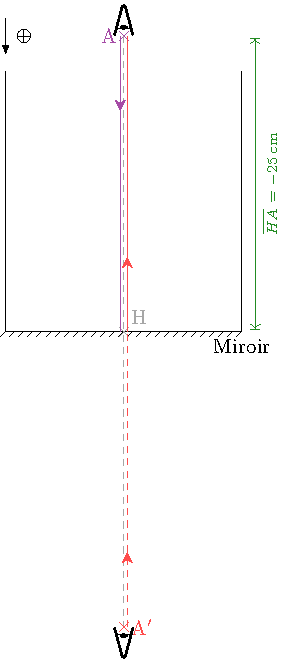
\includegraphics{ch2-5-1}
            \vfill
            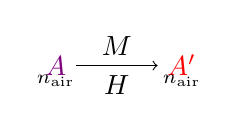
\begin{tikzpicture}
                % Réduit
                \node[] (A) at (-0.8,0) {\color{Purple}$A$};
                \node[below] at (A) {\scriptsize $n_{\rm air}$};
                \node[] (Ap) at (0.8,0) {\color{Red}$A'$};
                \node[below] at (Ap) {\scriptsize $n_{\rm air}$};
                \draw[->] (A) -- (Ap)
                    node [midway, above] {$M$}
                    node [midway, below] {$H$};
                %\node[below=0.3, Purple!70] (Ab) at (A) {$-infty$};
                %\node[below=0.3, brandeisblue] (A_1b) at (A_1) {$A_1 = F'_v$};
                %\node[below=0.3, ForestGreen] (A_1bb) at (A_1b) {$A_1 = R$};
                %\node[below=0.3, orange!70] (A_2b) at (A_2) {$A' = E$};
                %\draw[->, Purple!70] (Ab) to[bend right] (A_1b.west);
                %\draw[->, orange!70] (A_2b) to[bend left] (A_1bb.east);
            \end{tikzpicture}
        \end{center}
        \tcblower
        \begin{center}
            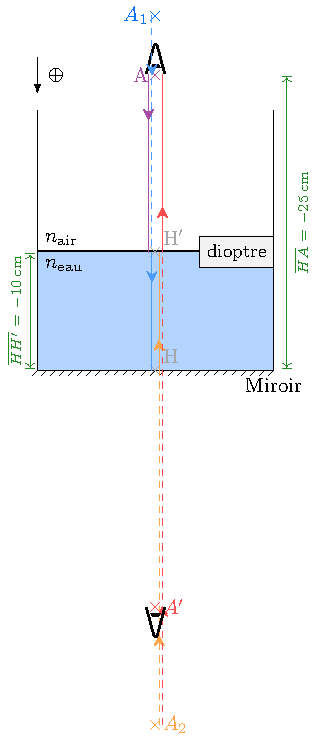
\includegraphics{ch2-5-2}
            \vfill
            \begin{tikzpicture}
                % Réduit
                \node[] (A) at (-2.4,0) {\color{Purple}$A$};
                \node[below] at (A) {\scriptsize $n_{\rm air}$};
                \node[] (A1) at (-0.8,0) {\color{brandeisblue}$A_1$};
                \node[below] at (A1) {\scriptsize $n_{\rm eau}$};
                \node[] (A2) at (0.8,0) {\color{orange}$A_2$};
                \node[below] at (A2) {\scriptsize $n_{\rm eau}$};
                \node[] (Ap) at (2.4,0) {\color{Red}$A'$};
                \node[below] at (Ap) {\scriptsize $n_{\rm air}$};
                \draw[->] (A) -- (A1)
                    node [midway, above] {$D$}
                    node [midway, below] {$H'$};
                \draw[->] (A1) -- (A2)
                    node [midway, above] {$M$}
                    node [midway, below] {$H$};
                \draw[->] (A2) -- (Ap)
                    node [midway, above] {$D$}
                    node [midway, below] {$H'$};
            \end{tikzpicture}
        \end{center}
    \end{NCdefi}
    \begin{tcolorbox}[blankest, raster multicolumn=1, space to=\myspace]
        \begin{tcbraster}[raster columns=1]
            \begin{NCprop}[add to natural height=\myspace]{Résultat attendu}
                Ici, on demande un changement par rapport à la situation sans
                eau. Il faut donc étudier les deux situations.
            \end{NCprop}
            \begin{NCdemo}{Outils du cours}
                Relation de conjugaison pour un miroir plan :
                \[\obar{HA'} = - \obar{HA}\]
                Relation de conjugaison d'un dioptre plan :
                \[ 0 = \frac{n_2}{\obar{HA'}} - \frac{n_1}{\obar{HA}} \]
            \end{NCdemo}
            \begin{NCror}{Important}
                Il est pratiquement obligé de donner les schémas optiques
                « réduits » (en bas des schémas ici).\smallbreak
                \textbf{Miroir} : image de l'autre côté.\smallbreak
                \textbf{Dioptre plan} : image du même côté.
            \end{NCror}
        \end{tcbraster}
    \end{tcolorbox}
\end{tcbraster}
\begin{NCexem}[sidebyside]{Application}
    Dans la première situation, \fbox{$\obar{HA'} = -\obar{HA} = \SI{25}{cm}$}.
    \tcblower

    Dans la seconde, $\obar{H'A_1} = n_{\rm eau}\obar{H'A} =
    \underline{\SI{-20}{cm}}$ avec $\obar{H'A} = \SI{-15}{cm}$
    d'abord.\smallbreak

    Ensuite $\obar{HA_2} = -\obar{HA_1} = \underline{\SI{30}{cm}}$ avec
    $\obar{HA_1} = -10-20 = \SI{-30}{cm}$.\smallbreak

    Finalement, $\obar{H'A'} = \frac{\obar{H'A_2}}{n_{\rm eau}} =
    \underline{\SI{30}{cm}}$ avec $\obar{H'A_2} = 10+30 =
    \SI{40}{cm}$.\smallbreak

    Autrement dit, \fbox{$\obar{HA'} = \SI{20}{cm}$} ; l'image s'est donc
    \textbf{rapprochée} de \SI{5}{cm}.
\end{NCexem}

\newpage

\section{Lois de Snell-Descartes}
Cet exercice est d'une simplicité absolue. Et pourtant...
\begin{tcbraster}[raster columns=5, raster equal height=rows]
    \begin{NCdefi}[raster multicolumn=3, sidebyside, righthand width=4cm]{Données}
        \begin{enumerate}
            \item Rayon incident sur un dioptre entre air et milieu d'indice $n$ :
                angle {\huge avec le dioptre} de \SI{56}{\degres} ;
            \item Différence d'angle entre rayon incident et réfléchi (« déviation
                ») de \SI{13.5}{\degres}.
        \end{enumerate}
        \tcblower
        \begin{center}
            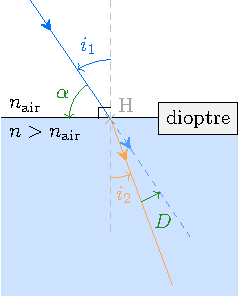
\includegraphics{ch2-6}
        \end{center}
    \end{NCdefi}    
    \begin{tcolorbox}[blankest, raster multicolumn=2, space to=\myspace]
        \begin{tcbraster}[raster columns=1]
            \begin{NCprop}[add to natural height=\myspace]{Résultat attendu}
                Indice du liquide.
            \end{NCprop}
            \begin{NCdemo}{Outils du cours}
                Loi de Snell-Descartes :
                \[ n_1\sin i_1 = n_2 \sin i_2 \]
                avec $n_1$ l'indice du milieu d'indidence, $n_2$ celui du milieu
                de réfraction, $i_1$ l'angle d'incidence et $i_2$ l'angle de
                réfraction.
            \end{NCdemo}
        \end{tcbraster}
    \end{tcolorbox}
\end{tcbraster}

\begin{NCexem}{Application}
    Un bon schéma fait attentivement est \textbf{nécessaire} ici. En effet,
    les angles donnés ne sont pas ceux qu'on utilise dans la relation de
    Snell-Descartes. \bigbreak
    
    En appelant $\alpha$ l'angle entre le rayon et le dioptre, on a
    \[ \alpha + i_1 = 90\degres\]
    donc \fbox{$i_1 = \SI{34}{\degres}$}. Et en appelant $D$ la déviation entre
    les deux rayons, on a
    \[ i_1 = i_2 + D\]
    soit \fbox{$i_2 = \SI{20.5}{\degres}$}. On en déduit donc
    \[\boxed{n = \frac{\sin i_1}{\sin i_2}} \quad \text{avec} \quad
        \left\{
            \begin{array}{rcl}
                i_1 & = & \SI{34}{\degres}\\
                i_2 & = & \SI{20.5}{\degres}
            \end{array}
    \right. \quad \text{soit} \quad \boxed{n = 1.6}
    \]
\end{NCexem}

\newpage

\setcounter{section}{8}
\section{Prisme rectangle}
\begin{tcbraster}[raster columns=3, raster equal height=rows]
    \begin{NCdefi}[raster multicolumn=2]{Schéma}
        \begin{center}
            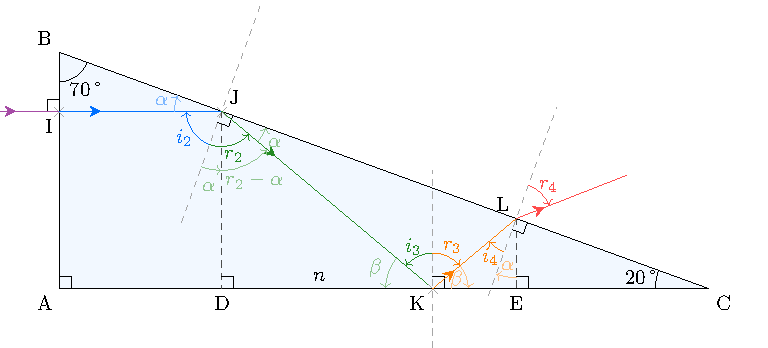
\includegraphics[scale=0.94]{ch2-9}
            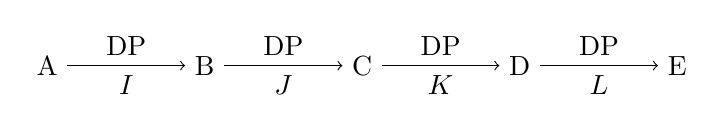
\begin{tikzpicture}[]
                \node[] (A) at (0,0) {A};
                \node[] (B) at (2,0) {B};
                \node[] (C) at (4,0) {C};
                \node[] (D) at (6,0) {D};
                \node[] (E) at (8,0) {E};
                \draw[->] (A) -- (B)
                    node [midway, above] {DP}
                    node [midway, below] {$I$};
                \draw[->] (B) -- (C)
                    node [midway, above] {DP}
                    node [midway, below] {$J$};
                \draw[->] (C) -- (D)
                    node [midway, above] {DP}
                    node [midway, below] {$K$};
                \draw[->] (D) -- (E)
                    node [midway, above] {DP}
                    node [midway, below] {$L$};
            \end{tikzpicture}
        \end{center}
    \end{NCdefi}
    \begin{tcolorbox}[blankest, raster multicolumn=1, space to=\myspace]
        \begin{tcbraster}[raster columns=1]
            \begin{NCprop}[]{Résultat attendu}
                On cherche à suivre le chemin du rayon indiqué dans l'énoncé. Il
                faut pour cela savoir ce qui peut arriver au rayon. Dans le cas
                du passage par un dioptre plan, il peut y avoir traversée du
                dioptre avec Snell-Descartes, ou réflexion dans le cas $n_2 <
                n_1$.
            \end{NCprop}
            \begin{NCdemo}{Outils du cours}
                Loi de Snell-Descartes :
                \[ n_1\sin i = n_2\sin r\]
                et pour $n_2 < n_1$, $i_\ell$ :
                \[ n_1\sin i_\ell = n_2\sin 90\degres = n_2\]
                tel que $i_1 > i_\ell$ est réfléchi.
            \end{NCdemo}
        \end{tcbraster}
    \end{tcolorbox}
\end{tcbraster}
\begin{NCexem}[sidebyside]{Application}
    Ici, l'angle limite de réflexion à l'intérieur du prisme est : \[i_\ell =
    \arcsin \frac{1}{n} = \boxed{\SI{41.8}{\degres}}\]
    \begin{description}
        \item[I] : $\boxed{i_1 = \SI{0}{\degres}}$ donc
            $\boxed{r_1 = \SI{0}{\degres}}$ ;
        \item[J] : Ici, on doit voir que $\alpha = \SI{20}{\degres}$ puisque
            dans le triangle BIJ, la somme des angles doit valoir $\SI{180}
            {\degres}$ et qu'on a un angle droit + un angle de \SI{70}{\degres}.
            On en déduit que $\boxed{i_2 = \SI{70}{\degres}}$ également, car
            $i_2 + \alpha = \SI{90}{\degres}$.\smallbreak
            Comme \underline{$i_2 > i_\ell$}, le rayon ne traverse pas mais est
            réfléchi, soit $\boxed{r_2 = \SI{70}{\degres}}$.
    \end{description}
    \tcblower
    \begin{description}
        \item[K] : Pour trouver l'angle en K, on peut par exemple chercher
            l'angle $\beta$ : en construisant le triangle rectangle JDK, on
            trouve que l'angle au sommet est $r_2 - \alpha = \SI{50}{\degres}$ ;
            avec l'angle droit en D, $\beta = \SI{40}{\degres}$, et $\boxed{i_3
                = \SI{50}{\degres} > i_\ell}$ donc rayon réfléchi $\boxed{r_3 =
            \SI{50}{\degres}}$.
        \item[L] : De même qu'en J, tracer LEC indique que $i_4 + \alpha + \beta
            = \SI{90}{\degres}$, soit $\boxed{i_4 = \SI{30}{\degres} < i_\ell}$
            : on applique donc Snell-Descartes ici, et on obtient
            \[\boxed{r_4} = \arcsin (n\times \sin i_4) =
            \boxed{\SI{48.6}{\degres}}\]
    \end{description}
\end{NCexem}
\end{document}
